\documentclass[11pt,a4paper]{article}

\usepackage[margin=2.5cm]{geometry}
\usepackage[T1]{fontenc}
\usepackage[utf8]{inputenc}
\usepackage{lmodern}
\usepackage{microtype}
\usepackage{amsmath,amssymb}
\usepackage{booktabs}
\usepackage{graphicx}
\usepackage[hidelinks]{hyperref}

\setcounter{tocdepth}{1}

% Register numbered report headings without rendering empty body sections.
\newcommand{\tocsection}[1]{%
  \refstepcounter{section}%
  \addcontentsline{toc}{section}{\protect\numberline{\thesection}#1}}
\newcommand{\tocsubsection}[1]{%
  \refstepcounter{subsection}%
  \addcontentsline{toc}{subsection}{\protect\numberline{\thesubsection}#1}}
\newcommand{\tocsubsubsection}[1]{%
  \refstepcounter{subsubsection}%
  \addcontentsline{toc}{subsubsection}{\protect\numberline{\thesubsubsection}#1}}
\newcommand{\tocunnumberedsection}[1]{%
  \phantomsection%
  \addcontentsline{toc}{section}{#1}}

\title{Stability and Bifurcation of a Simple Food Chain\\
in a Chemostat with Removal Rates}
\author{Mathematical Modelling Project Group}
\date{\today}

\begin{document}

\hypersetup{pageanchor=false}
\begin{titlepage}

% \thispagestyle{empty}
% \thisfancypage{
% \fbox}{} 
\begin{center}

\textbf{HANOI UNIVERSITY OF SCIENCE AND TECHNOLOGY}\\
\textbf{SCHOOL OF INFORMATION AND COMMUNICATION TECHNOLOGY}\\[1cm]


\includegraphics[width=10cm]{images/SOICT-HUST.png}\\[1cm]

\textbf{\huge{PROJECT REPORT}}\\[0.5cm]
% \textbf{\Large{Introduction to Artificial Intelligence}}\\[1cm]

% \setlength{\baselineskip}{2\baselineskip}
{\textbf{\Large{Stability and Bifurcation of a Simple Food Chain
in a Chemostat with Removal Rates}}}\\[1cm]

{\large{\textbf{Course:} Math Modeling}}\\
{\large{\textbf{Mentor:} Dr. Bui Quoc Trung}}\\[2cm]

%\vspace{2cm}
% Please add the following required packages to your document preamble:
\begin{tabular}{@{}l@{\hspace{3cm}}c@{}}
    \textit{Authors:} & Student ID: \\ 
    ho va ten & mssv \\ 
    
\end{tabular}
\vspace{1cm}
\vfill
\large{Hanoi, June 2026}

\end{center}
\end{titlepage}

\clearpage

\hypersetup{pageanchor=true}
\pagenumbering{roman}
\tableofcontents
\clearpage
\pagenumbering{arabic}

\tocsection{Introduction}
\tocsubsection{Introduction to the Problem}
\tocsubsubsection{Chemostats and Food-Chain Dynamics}
\tocsubsubsection{Biological Problem and Research Questions}
\tocsubsubsection{Project Objectives}
\tocsubsubsection{Scope of the Study}

\tocsubsection{Modeling Approach}
\tocsubsubsection{Continuous-Time Ordinary Differential Equation Model}
\tocsubsubsection{Biological Assumptions}
\tocsubsubsection{Monod Functional Responses}
\tocsubsubsection{Reasons for Selecting This Approach}
\tocsubsubsection{Connection to the Mathematical Modeling Process}

\section{Mathematical Model and Theory}
\label{sec:mathematical-model}

The reference first formulates the food chain in dimensional variables and
then rescales concentration and time.  Nutrient concentration is measured
relative to the input concentration, time is measured in units of the inverse
chemostat dilution rate, and the organism concentrations are scaled using the
corresponding yield constants.  This nondimensionalization fixes the nutrient
input and dilution terms at one and reduces the model to four state variables
and three effective removal rates.  The model used in the analysis and in our
implementation is
\begin{equation}
\label{eq:model}
\begin{aligned}
\dot S &= 1-S-f_1(S)x,\\
\dot x &= x\bigl(f_1(S)-D_1\bigr)-f_2(x)y,\\
\dot y &= y\bigl(f_2(x)-D_2\bigr)-f_3(y)z,\\
\dot z &= z\bigl(f_3(y)-D_3\bigr).
\end{aligned}
\end{equation}
Here and below a dot denotes differentiation with respect to dimensionless
time.

\subsection{State Variables and Model Parameters}

The variables form the state vector
\(
X(t)=(S(t),x(t),y(t),z(t))^{\mathsf T}\in\mathbb{R}_+^4
\).
Their meanings are summarized in Table~\ref{tab:model-variables}.

\begin{table}[htbp]
\centering
\caption{State variables of the nondimensional chemostat model.}
\label{tab:model-variables}
\begin{tabular}{cll}
\toprule
Symbol & Biological meaning & Domain \\
\midrule
\(S(t)\) & Nutrient concentration & \(S\geq 0\) \\
\(x(t)\) & Prey concentration; consumes the nutrient & \(x\geq 0\) \\
\(y(t)\) & First-predator concentration; consumes \(x\) & \(y\geq 0\) \\
\(z(t)\) & Top-predator concentration; consumes \(y\) & \(z\geq 0\) \\
\bottomrule
\end{tabular}
\end{table}

The paper allows general response functions \(f_i\).  It assumes that every
\(f_i:\mathbb{R}_+\rightarrow\mathbb{R}_+\) is continuously differentiable,
\(f_i(0)=0\), and \(f_i'(u)>0\) for \(u>0\).  Thus, growth increases with the
available food concentration.  For reproducible simulations, the project
specializes these functions to the Monod form
\begin{equation}
\label{eq:monod}
f_i(u)=\frac{a_i u}{k_i+u},\qquad a_i>0,\quad k_i>0,qquad i=1,2,3.
\end{equation}
The parameter \(a_i\) is the maximum specific growth rate and \(k_i\) is the
half-saturation constant, since \(f_i(k_i)=a_i/2\).  The derivative and inverse
needed in the equilibrium calculations are
\begin{equation}
\label{eq:monod-derivative-inverse}
f_i'(u)=\frac{a_i k_i}{(k_i+u)^2},
\qquad
f_i^{-1}(d)=\frac{d k_i}{a_i-d}\quad (0\leq d<a_i).
\end{equation}

Each \(D_i>0\) is the dimensionless total removal rate of one organism.  In
the dimensional model this rate is the sum of chemostat washout and the
organism's specific death rate; division by the dilution rate produces the
dimensionless \(D_i\).  The nine numerical parameters used by the simulator
are therefore
\[
(a_1,k_1,a_2,k_2,a_3,k_3,D_1,D_2,D_3).
\]

\subsection{Governing Differential Equations}

The first equation of~\eqref{eq:model} balances normalized nutrient inflow,
nutrient washout, and consumption by the prey.  The prey grows at per-capita
rate \(f_1(S)\), is removed at rate \(D_1\), and is consumed by the first
predator through the flux \(f_2(x)y\).  Similarly, \(y\) grows through prey
consumption, is removed at rate \(D_2\), and is consumed by \(z\).  The top
predator grows at rate \(f_3(y)\) and is removed at rate \(D_3\).

This chain structure is important: \(y\) does not consume nutrient directly,
and \(z\) consumes neither nutrient nor prey.  The transfer terms cancel when
all four equations are added.  Distinct removal rates prevent the stronger
conservation law available in equal-removal chemostat models, so the complete
four-dimensional system must be studied.

\subsection{Initial Conditions and Parameter Restrictions}

The reference considers strictly positive initial data,
\begin{equation}
\label{eq:initial-condition}
S(0)=S_0>0,\qquad x(0)=x_0>0,\qquad
y(0)=y_0>0,\qquad z(0)=z_0>0.
\end{equation}
Boundary initial states are also meaningful when studying washout equilibria.
All model parameters are positive.  In addition, a finite positive solution
of \(f_i(u)=D_i\) requires \(D_i<a_i\) for the Monod functions.  Stronger
conditions are needed for an equilibrium to lie in the biologically feasible
region; these are derived below rather than imposed globally.

\subsection{Nonnegativity, Boundedness, and Biological Feasibility}

The nonnegative orthant is positively invariant.  At \(S=0\), the first
equation gives \(\dot S=1>0\).  At \(x=0\), \(y=0\), or \(z=0\), the
corresponding derivative is zero because \(f_i(0)=0\).  Therefore a solution
starting with nonnegative concentrations cannot cross into negative values.

To establish boundedness, define the total dimensionless concentration
\[
T(t)=S(t)+x(t)+y(t)+z(t).
\]
Adding the equations in~\eqref{eq:model} gives
\begin{equation}
\label{eq:total-biomass}
\dot T=1-S-D_1x-D_2y-D_3z.
\end{equation}
Let
\[
D_{\min}=\min\{1,D_1,D_2,D_3\},\qquad
D_{\max}=\max\{1,D_1,D_2,D_3\}.
\]
Since all state variables are nonnegative,
\begin{equation}
1-D_{\max}T\leq \dot T\leq 1-D_{\min}T.
\end{equation}
The scalar comparison theorem consequently yields
\begin{equation}
\frac{1}{D_{\max}}
\leq \liminf_{t\to\infty}T(t)
\leq \limsup_{t\to\infty}T(t)
\leq \frac{1}{D_{\min}}.
\end{equation}
Equivalently, for any sufficiently small \(\kappa>0\), trajectories are
eventually attracted to the bounded region
\begin{equation}
\label{eq:absorbing-region}
\Gamma_\kappa=
\left\{X\in\mathbb{R}_+^4:
\frac{1}{D_{\max}}-\kappa\leq S+x+y+z
\leq\frac{1}{D_{\min}}+\kappa\right\}.
\end{equation}
Thus the model is dissipative: long-term trajectories enter a common bounded
set.  This result is both biologically necessary and numerically useful,
because an unbounded simulated trajectory would indicate an invalid parameter
or integration failure rather than intended model behavior.

\subsection{Equilibrium Points}

An equilibrium \(P=(S^*,x^*,y^*,z^*)\) satisfies
\begin{equation}
\label{eq:equilibrium-system}
\begin{aligned}
1-S^*-f_1(S^*)x^*&=0,\\
x^*\bigl(f_1(S^*)-D_1\bigr)-f_2(x^*)y^*&=0,\\
y^*\bigl(f_2(x^*)-D_2\bigr)-f_3(y^*)z^*&=0,\\
z^*\bigl(f_3(y^*)-D_3\bigr)&=0.
\end{aligned}
\end{equation}
The four possible trophic regimes follow by deciding which organism
concentrations are zero.

\subsubsection{Washout Equilibrium \(P_0\)}

If all organisms are absent, nutrient converges to its normalized input level:
\begin{equation}
P_0=(1,0,0,0).
\end{equation}
This equilibrium always exists.

\subsubsection{Prey-Only Equilibrium \(P_1\)}

For \(x_1>0\) and \(y_1=z_1=0\), the prey equation requires
\(f_1(S_1)=D_1\).  The nutrient balance then gives
\begin{equation}
\label{eq:p1}
P_1=(S_1,x_1,0,0),\qquad
S_1=f_1^{-1}(D_1),\qquad
x_1=\frac{1-S_1}{D_1}.
\end{equation}
For Monod growth,
\begin{equation}
S_1=\frac{D_1k_1}{a_1-D_1}.
\end{equation}
The biological condition \(0<S_1<1\) is equivalent to
\(D_1<f_1(1)=a_1/(k_1+1)\).  This is precisely the condition that prey can
increase when rare at \(P_0\).

\subsubsection{Two-Species Equilibrium \(P_2\)}

For prey and the first predator to persist while \(z=0\), the \(y\)-equation
requires \(f_2(x_2)=D_2\).  Therefore
\begin{equation}
\label{eq:p2}
\begin{aligned}
P_2&=(S_2,x_2,y_2,0),\\
x_2&=f_2^{-1}(D_2),\\
S_2+f_1(S_2)x_2&=1,\\
y_2&=\frac{x_2\bigl(f_1(S_2)-D_1\bigr)}{D_2}.
\end{aligned}
\end{equation}
For the Monod function, \(x_2=D_2k_2/(a_2-D_2)\).  Once \(x_2\) is known,
the equation for \(S_2\) has a unique root in \((0,1)\), because
\(S+f_1(S)x_2\) is strictly increasing from zero to a value greater than one.
Finally, \(y_2>0\) requires \(f_1(S_2)>D_1\).  In the equilibrium hierarchy,
this condition is equivalent to the first-predator invasion threshold
\(f_2(x_1)>D_2\).

\subsubsection{Coexistence Equilibrium \(P_3\)}

At an interior equilibrium all four components are positive.  The top-predator
equation first fixes
\begin{equation}
\label{eq:y3}
y_3=f_3^{-1}(D_3)
=\frac{D_3k_3}{a_3-D_3}
\end{equation}
for Monod growth.  The remaining coordinates satisfy
\begin{equation}
\label{eq:p3}
\begin{aligned}
P_3&=(S_3,x_3,y_3,z_3),\\
S_3+f_1(S_3)x_3&=1,\\
x_3\bigl(f_1(S_3)-D_1\bigr)&=f_2(x_3)y_3,\\
z_3&=\frac{y_3\bigl(f_2(x_3)-D_2\bigr)}{D_3}.
\end{aligned}
\end{equation}
The coupled equations for \(S_3\) and \(x_3\) generally do not have a useful
closed form, even after choosing Monod functions.  The implementation solves
\(S+f_1(S)x=1\) by bisection for each trial \(x\), then locates a sign change
in the prey-balance residual.  The coexistence state is feasible only when all
coordinates are positive.  In particular, \(D_3<a_3\) is needed to define
\(y_3\), and \(f_2(x_3)>D_2\) is needed for \(z_3>0\).

\subsection{Existence and Positivity Conditions}

The equilibria form a trophic hierarchy controlled by invasion rates.  An
invasion rate is the per-capita growth rate of a missing species when that
species is introduced at very low concentration.  The three relevant rates
are
\begin{equation}
\label{eq:invasion-rates}
\lambda_x=f_1(1)-D_1,\qquad
\lambda_y=f_2(x_1)-D_2,\qquad
\lambda_z=f_3(y_2)-D_3.
\end{equation}

\begin{table}[htbp]
\centering
\caption{Equilibrium hierarchy and biological existence conditions.}
\label{tab:equilibrium-existence}
\begin{tabular}{lll}
\toprule
Equilibrium & Persisting organisms & Main feasibility condition \\
\midrule
\(P_0\) & None & Always exists \\
\(P_1\) & \(x\) & \(\lambda_x>0\) \\
\(P_2\) & \(x,y\) & \(P_1\) exists and \(\lambda_y>0\) \\
\(P_3\) & \(x,y,z\) & \(P_2\) exists and \(\lambda_z>0\) \\
\bottomrule
\end{tabular}
\end{table}

Positive invasion means that the next trophic level can enter the lower-level
equilibrium.  Negative invasion means that it washes out when rare.  At a zero
invasion rate the corresponding equilibrium is nonhyperbolic, and a change in
the qualitative survival regime may occur.

\subsection{Local Stability and Threshold Conditions}

Linearizing~\eqref{eq:model} at a state \((S,x,y,z)\) gives the Jacobian
\begin{equation}
\label{eq:jacobian}
J=\begin{pmatrix}
-1-f_1'(S)x & -f_1(S) & 0 & 0\\
f_1'(S)x & f_1(S)-D_1-f_2'(x)y & -f_2(x) & 0\\
0 & f_2'(x)y & f_2(x)-D_2-f_3'(y)z & -f_3(y)\\
0 & 0 & f_3'(y)z & f_3(y)-D_3
\end{pmatrix}.
\end{equation}
An equilibrium is locally asymptotically stable when every eigenvalue of its
Jacobian has negative real part.

\paragraph{Stability of \(P_0\).}
At washout, the eigenvalues are
\begin{equation}
-1,\qquad f_1(1)-D_1,\qquad -D_2,\qquad -D_3.
\end{equation}
Consequently,
\begin{equation}
\label{eq:p0-stability}
P_0\text{ is locally asymptotically stable}
\quad\Longleftrightarrow\quad f_1(1)-D_1<0.
\end{equation}
For Monod growth this becomes
\(a_1/(k_1+1)<D_1\).  If the inequality is reversed, prey can invade and
\(P_0\) is unstable in the \(x\)-direction.

\paragraph{Stability of \(P_1\).}
The \((S,x)\) block of \(J(P_1)\) is
\[
J_{Sx}(P_1)=
\begin{pmatrix}
-1-x_1f_1'(S_1)&-D_1\\
x_1f_1'(S_1)&0
\end{pmatrix}.
\]
Its trace is negative and its determinant is positive, so both eigenvalues
have negative real part.  The remaining eigenvalues are
\(
f_2(x_1)-D_2
\)
and \(-D_3\).  Hence
\begin{equation}
\label{eq:p1-stability}
P_1\text{ is locally asymptotically stable}
\quad\Longleftrightarrow\quad f_2(x_1)-D_2<0.
\end{equation}
When this threshold is positive, \(P_1\) is a saddle that repels trajectories
in the \(y\)-direction.

\paragraph{Stability of \(P_2\).}
For a compact Routh--Hurwitz representation, define
\begin{align*}
a&=1+x_2f_1'(S_2), & b&=f_1(S_2), & c&=x_2f_1'(S_2),\\
d&=y_2f_2'(x_2), & e&=D_2, &
r&=f_1(S_2)-D_1-y_2f_2'(x_2).
\end{align*}
The active \((S,x,y)\) block is
\[
\begin{pmatrix}
-a&-b&0\\
c&r&-e\\
0&d&0
\end{pmatrix},
\]
whose characteristic polynomial is
\begin{equation}
\lambda^3+A_1\lambda^2+A_2\lambda+A_3,
\end{equation}
with
\begin{equation}
\label{eq:p2-cubic-coefficients}
A_1=a-r,\qquad
A_2=ed-ar+bc,\qquad
A_3=aed.
\end{equation}
The fourth eigenvalue is the top-predator invasion rate
\(\lambda_z=f_3(y_2)-D_3\).  The cubic Routh--Hurwitz criterion gives
\begin{equation}
\label{eq:p2-stability}
A_1>0,\quad A_2>0,\quad A_3>0,\quad A_1A_2>A_3,
\quad\text{and}\quad f_3(y_2)-D_3<0
\end{equation}
as sufficient and necessary local stability conditions.  If the active block
is stable but \(f_3(y_2)-D_3>0\), then \(P_2\) is a saddle repelling in the
\(z\)-direction.

\paragraph{Stability of \(P_3\).}
At coexistence, introduce the abbreviations
\begin{align*}
A&=1+x_3f_1'(S_3), & B&=f_1(S_3), & C&=x_3f_1'(S_3),\\
R&=f_1(S_3)-D_1-y_3f_2'(x_3),
& E&=f_2(x_3), & F&=y_3f_2'(x_3),\\
Q&=f_2(x_3)-D_2-z_3f_3'(y_3),
& G&=f_3(y_3), & H&=z_3f_3'(y_3).
\end{align*}
Then
\begin{equation}
J(P_3)=
\begin{pmatrix}
-A&-B&0&0\\
C&R&-E&0\\
0&F&Q&-G\\
0&0&H&0
\end{pmatrix}.
\end{equation}
Set \(p=A-R\) and \(q=BC-AR\).  Expanding
\(\det(\lambda I-J(P_3))\) gives
\begin{equation}
\lambda^4+C_1\lambda^3+C_2\lambda^2+C_3\lambda+C_4,
\end{equation}
where
\begin{equation}
\label{eq:p3-quartic-coefficients}
\begin{aligned}
C_1&=p-Q,\\
C_2&=q-Qp+EF+GH,\\
C_3&=EFA-Qq+GHp,\\
C_4&=GHq.
\end{aligned}
\end{equation}
The quartic Routh--Hurwitz conditions are
\begin{equation}
\label{eq:p3-stability}
\begin{gathered}
C_1>0,\quad C_2>0,\quad C_3>0,\quad C_4>0,\\
C_1C_2>C_3,\qquad
C_1C_2C_3>C_3^2+C_1^2C_4.
\end{gathered}
\end{equation}
These inequalities provide a direct analytical or numerical test for local
coexistence stability.

\subsection{Persistence and Bifurcation Behavior}

Local stability describes trajectories close to one equilibrium, whereas
uniform persistence concerns all positive solutions.  The reference combines
the dissipativity result with boundary-flow arguments.  In particular, if
\(P_1\) is globally attracting on the \((S,x)\) boundary subsystem but repels
the missing first predator, and \(P_2\) is globally attracting on the
\((S,x,y)\) boundary subsystem but repels the missing top predator, then no
strictly positive trajectory can approach the boundary.  Under the paper's
additional hyperbolicity and no-cycle assumptions, there is an \(\eta>0\)
such that
\begin{equation}
\liminf_{t\to\infty}S(t),\quad
\liminf_{t\to\infty}x(t),\quad
\liminf_{t\to\infty}y(t),\quad
\liminf_{t\to\infty}z(t)\geq\eta.
\end{equation}
This uniform persistence implies the existence of at least one positive
interior equilibrium \(P_3\).

For bifurcation analysis, the paper introduces a real parameter \(\mu\) into
the prey growth response, writing \(f_1(S;\mu)\), and studies how the Jacobian
eigenvalues change with \(\mu\).  A Hopf bifurcation requires a complex
conjugate pair to cross the imaginary axis with nonzero speed while the other
eigenvalues remain away from it.

At \(P_2\), the cubic factor reaches a candidate Hopf boundary when
\begin{equation}
\label{eq:p2-hopf-boundary}
A_1A_2=A_3,
\end{equation}
with positive coefficients, a nonzero top-predator eigenvalue, and the
transversality condition satisfied.  At \(P_3\), the corresponding quartic
boundary is
\begin{equation}
\label{eq:p3-hopf-boundary}
C_1C_2C_3=C_3^2+C_1^2C_4,
\end{equation}
again together with coefficient positivity and transversality.  Crossing one
of these boundaries can create a family of periodic solutions.  The numerical
oscillatory experiment later in this report illustrates behavior near such a
boundary, but a damped oscillatory trajectory alone is not a proof of Hopf
bifurcation.

\subsection{Consistency of the Implemented Model with the Reference Analysis}

Two inconsistencies in the printed article must be handled explicitly.  First,
the displayed nondimensional equation~(1.2) appears to repeat population
factors inside several per-capita growth terms.  Read literally, that display
does not produce the paper's later Jacobian or equilibrium formulas.  The
system in~\eqref{eq:model} does produce them and is therefore the model used by
the simulator, equilibrium calculations, and this report.  Second, the final
discussion states the opposite sign for washout stability, while Theorem~2.2
and the eigenvalues at \(P_0\) correctly require
\(f_1(1)-D_1<0\).  We follow the theorem and the direct linearization.

The code mirrors the mathematical construction as follows:
\begin{itemize}
\item \texttt{equilibria\_stability/model.py} implements~\eqref{eq:monod},
      its derivative, and its inverse;
\item \texttt{equilibria\_stability/analysis.py} computes \(P_0\) through
      \(P_3\), checks positivity, and evaluates the \(P_0\) threshold;
\item \texttt{demo/app.py} evaluates~\eqref{eq:jacobian} and computes its
      characteristic roots for the interactive local-stability display.
\end{itemize}

Table~\ref{tab:equilibrium-code-check} gives representative outputs produced
by the equilibrium implementation.  They also serve as analytical targets for
the simulations in Section~4.

\begin{table}[htbp]
\centering
\caption{Representative equilibrium calculations from the implemented model.}
\label{tab:equilibrium-code-check}
\small
\begin{tabular}{lll}
\toprule
Scenario & Richest feasible equilibrium & Coordinates \((S,x,y,z)\) \\
\midrule
Washout & \(P_0\) & \((1,0,0,0)\) \\
Prey only & \(P_1\) & \((0.166667,1.666667,0,0)\) \\
Two species & \(P_2\) & \((0.628667,0.333333,0.409333,0)\) \\
Coexistence & \(P_3\) & \((0.055067,0.804597,0.280534,0.081550)\) \\
\bottomrule
\end{tabular}
\end{table}

\tocsection{Solving Algorithm and Simulator Implementation}
\tocsubsection{Numerical Initial-Value Problem}
\tocsubsection{Right-Hand-Side Evaluation}
\tocsubsection{Euler Method}
\tocsubsection{Fourth-Order Runge--Kutta Method}
\tocsubsection{Simulation Algorithm}
\tocsubsection{Input Parameters and Initial State}
\tocsubsection{CSV and Diagnostic Outputs}
\tocsubsection{Equilibrium and Outcome Classification}
\tocsubsection{Numerical Validation and Testing}
\tocsubsection{Reproducibility and Software Structure}

\section{Simulation Experiments and Results}

\subsection{Experimental Setup}

The purpose of the simulation experiments is to connect the analytical
equilibria of the chemostat food-chain model with visible long-time dynamics.
All runs use the internally consistent four-dimensional model
\[
\begin{aligned}
\frac{dS}{dt} &= 1-S-f_1(S)x,\\
\frac{dx}{dt} &= x(f_1(S)-D_1)-f_2(x)y,\\
\frac{dy}{dt} &= y(f_2(x)-D_2)-f_3(y)z,\\
\frac{dz}{dt} &= z(f_3(y)-D_3),
\end{aligned}
\]
where \(S\) is the nutrient concentration, \(x\) is the prey population,
\(y\) is the first predator, and \(z\) is the top predator. The response
functions are Monod functions,
\[
f_i(u)=\frac{a_i u}{k_i+u}, \qquad i=1,2,3.
\]
This version of the system is the one used in the equilibrium and Jacobian
analysis. It was also used by the simulator so that the numerical experiments
and the theoretical formulas describe the same model.

The trajectories were computed with the classical fourth-order Runge--Kutta
method using time step \(\Delta t=0.01\). The initial condition was fixed at
\[
(S_0,x_0,y_0,z_0)=(0.5,0.2,0.1,0.05)
\]
for all five main experiments. The four equilibrium scenarios \(P_0\) through
\(P_3\) were integrated until \(t=500\). The oscillatory case was integrated
until \(t=2000\), because its transient oscillations decay slowly and a shorter
run could give a misleading classification. The simulator wrote every tenth
time step to CSV files and recorded diagnostics including final states,
componentwise minima and maxima, negative-state clamps, explosion status, and
distances from the analytical equilibria. No run exploded and no run required
negative-state clamping.

\begin{figure}[htbp]
    \centering
    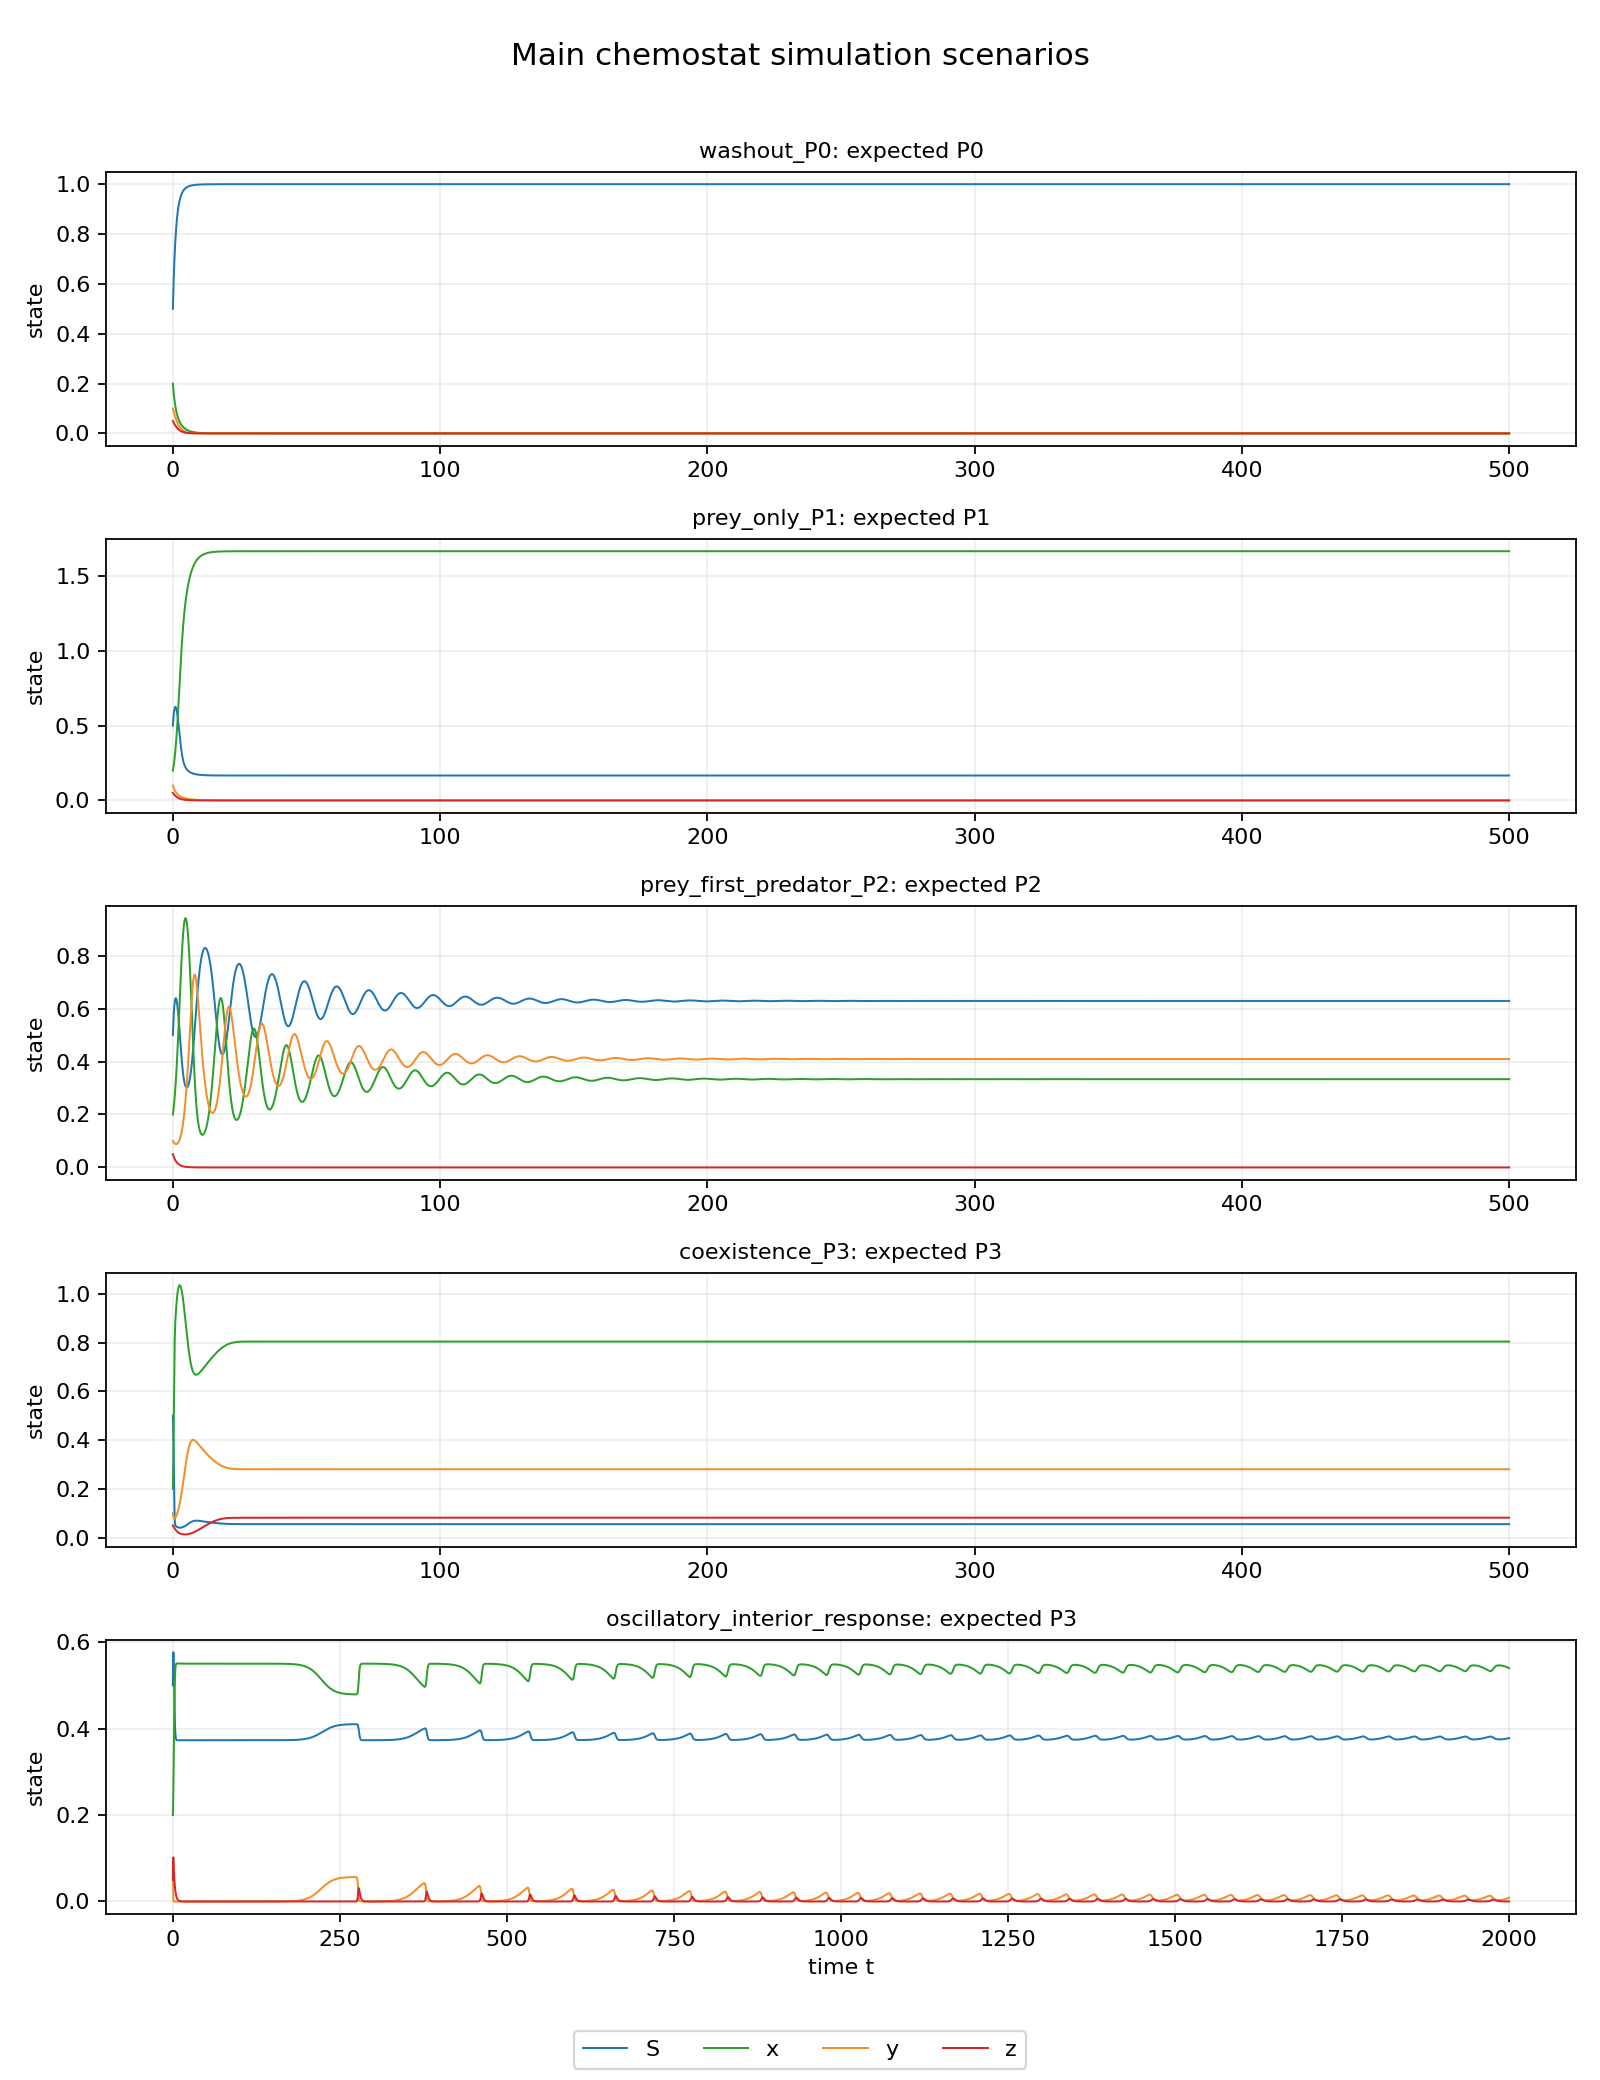
\includegraphics[width=0.95\textwidth]{results/main_scenarios/main_scenarios_overview.png}
    \caption{Overview of the five main simulation regimes generated by the RK4 simulator.}
    \label{fig:main-scenarios-overview}
\end{figure}

\subsection{Parameter-Set Selection}

Five parameter sets were selected to represent the main biological regimes
predicted by the equilibrium hierarchy: complete washout \(P_0\), prey-only
survival \(P_1\), survival of the prey and first predator \(P_2\), coexistence
of all trophic levels \(P_3\), and a slowly damped oscillatory response near
an interior equilibrium. The values used in the simulations are listed in
Table~\ref{tab:main-scenario-parameters}.

\begin{table}[htbp]
\centering
\caption{Parameter sets used in the main simulation experiments.}
\label{tab:main-scenario-parameters}
\resizebox{\textwidth}{!}{%
\begin{tabular}{lccccccccc}
\hline
Scenario & \(a_1\) & \(k_1\) & \(a_2\) & \(k_2\) & \(a_3\) & \(k_3\) & \(D_1\) & \(D_2\) & \(D_3\)\\
\hline
\(P_0\) washout & 0.60 & 0.50 & 1.50 & 0.50 & 1.20 & 0.40 & 0.80 & 0.70 & 0.70\\
\(P_1\) prey only & 2.00 & 0.50 & 0.50 & 1.00 & 1.00 & 1.00 & 0.50 & 0.60 & 0.60\\
\(P_2\) two species & 2.00 & 0.50 & 2.00 & 1.00 & 0.50 & 1.00 & 0.50 & 0.50 & 0.70\\
\(P_3\) coexistence & 4.80 & 0.17 & 4.30 & 1.85 & 4.60 & 1.66 & 0.72 & 1.11 & 0.665\\
Oscillatory response & 6.52 & 1.76 & 5.07 & 2.64 & 3.78 & 0.0466 & 1.14 & 0.778 & 0.488\\
\hline
\end{tabular}%
}
\end{table}

\subsection{Washout Scenario P0}

In the washout scenario, the numerical solution converged to
\[
(S,x,y,z)\approx(1,0,0,0),
\]
with distance \(5.55\times 10^{-15}\) from the analytical equilibrium \(P_0\).
Biologically, this means that the prey cannot grow fast enough on the incoming
nutrient to overcome its removal rate. Once the prey disappears, both predator
populations also disappear because their food sources are absent. The nutrient
therefore returns to its normalized input concentration.

\begin{figure}[htbp]
    \centering
    
\includegraphics[width=0.88\textwidth]{results/main_scenarios/washout_P0_timeseries.png}
    \caption{Running simulation image for the washout scenario \(P_0\).}
    \label{fig:washout-p0-timeseries}
\end{figure}

\subsection{Prey-Only Scenario P1}

In the prey-only scenario, the final numerical state was
\[
(S,x,y,z)\approx(0.166667,1.666667,0,0),
\]
with distance \(2.57\times 10^{-14}\) from the theoretical equilibrium \(P_1\).
The prey population survives because it can exploit the nutrient supply, but
the resulting prey concentration is not sufficient for the first predator to
overcome its own removal rate. Consequently both predators wash out. The
nutrient level is much lower than in \(P_0\), showing that prey persistence is
associated with continuous nutrient consumption.

\begin{figure}[htbp]
    \centering
    
\includegraphics[width=0.88\textwidth]{results/main_scenarios/prey_only_P1_timeseries.png}
    \caption{Running simulation image for the prey-only scenario \(P_1\).}
    \label{fig:prey-only-p1-timeseries}
\end{figure}

\subsection{Two-Species Scenario P2}

In the two-species scenario, the solution approached
\[
(S,x,y,z)\approx(0.628666,0.333334,0.409333,0),
\]
which is \(1.29\times 10^{-6}\) from the analytical equilibrium \(P_2\). The
prey and first predator persist, while the top predator is removed from the
system. This confirms the expected intermediate regime in which the first
predator can invade the prey-only equilibrium, but the second predator cannot
invade the prey--predator equilibrium. The approach to \(P_2\) contains small
damped transients, so temporary oscillation should not be confused with
sustained periodic behavior.

\begin{figure}[htbp]
    \centering
    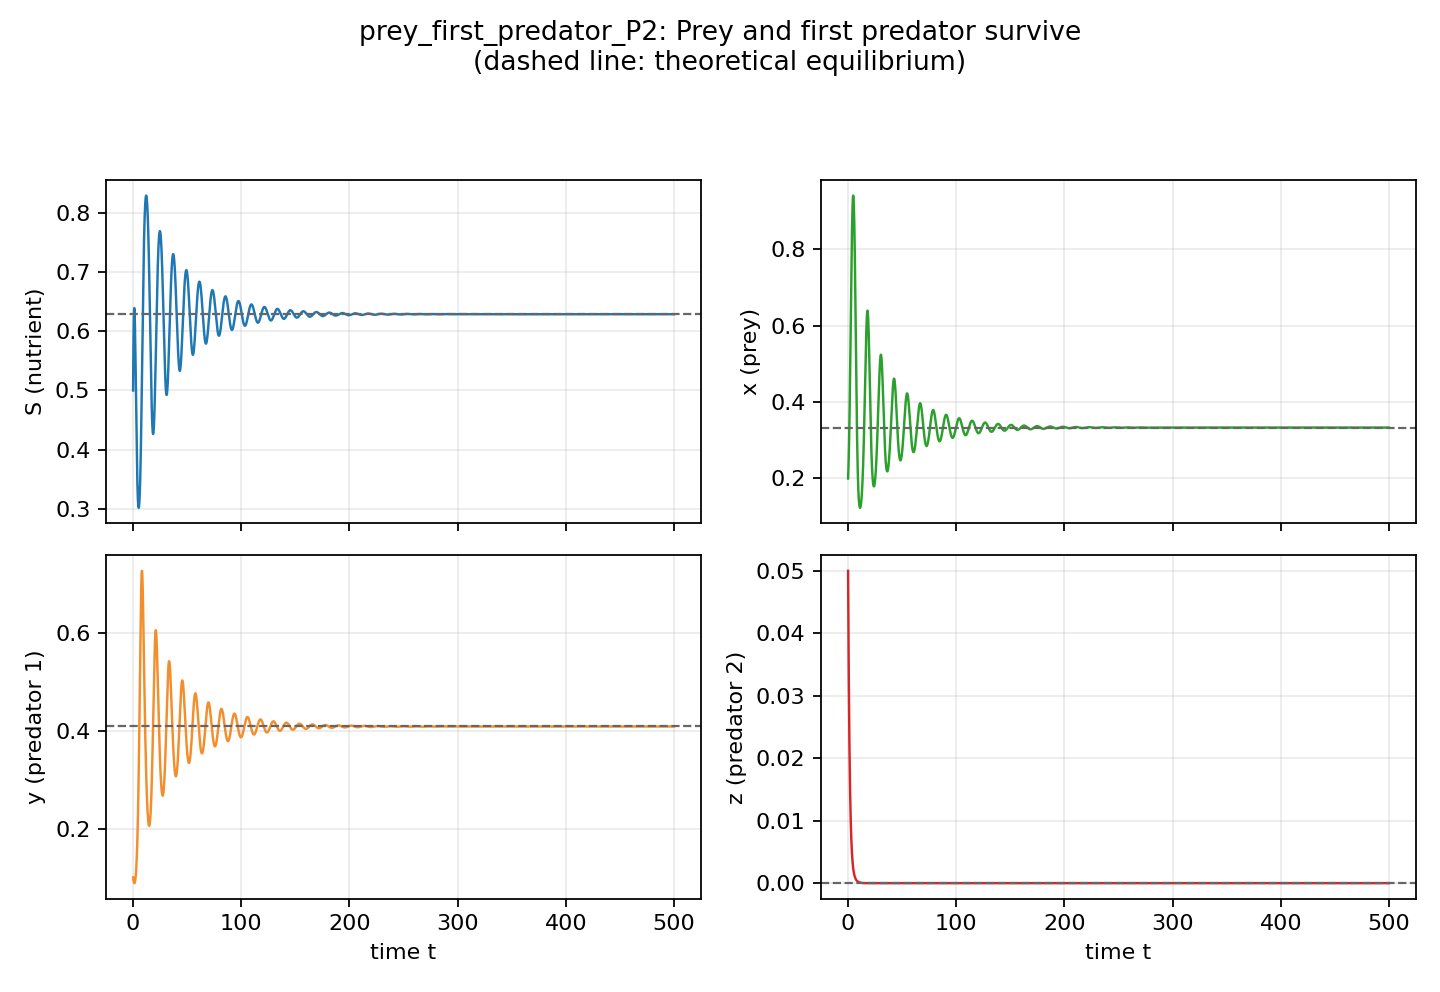
\includegraphics[width=0.88\textwidth]{results/main_scenarios/prey_first_predator_P2_timeseries.png}
    \caption{Running simulation image for the two-species scenario \(P_2\).}
    \label{fig:two-species-p2-timeseries}
\end{figure}

\subsection{Coexistence Scenario P3}

In the coexistence scenario, all state variables converged to positive values:
\[
(S,x,y,z)\approx(0.055067,0.804597,0.280534,0.081550).
\]
The distance from the analytical coexistence equilibrium \(P_3\) was
\(1.94\times 10^{-11}\). This close agreement shows that the simulator
reproduces the expected interior equilibrium for the selected parameter set.
In biological terms, nutrient enters the chemostat continuously, the prey
consumes nutrient, the first predator consumes prey, and the top predator
consumes the first predator. This numerical result supports the persistence
interpretation in the reference, although a single trajectory is not a proof
of uniform persistence for all admissible positive initial conditions.

\begin{figure}[htbp]
    \centering
    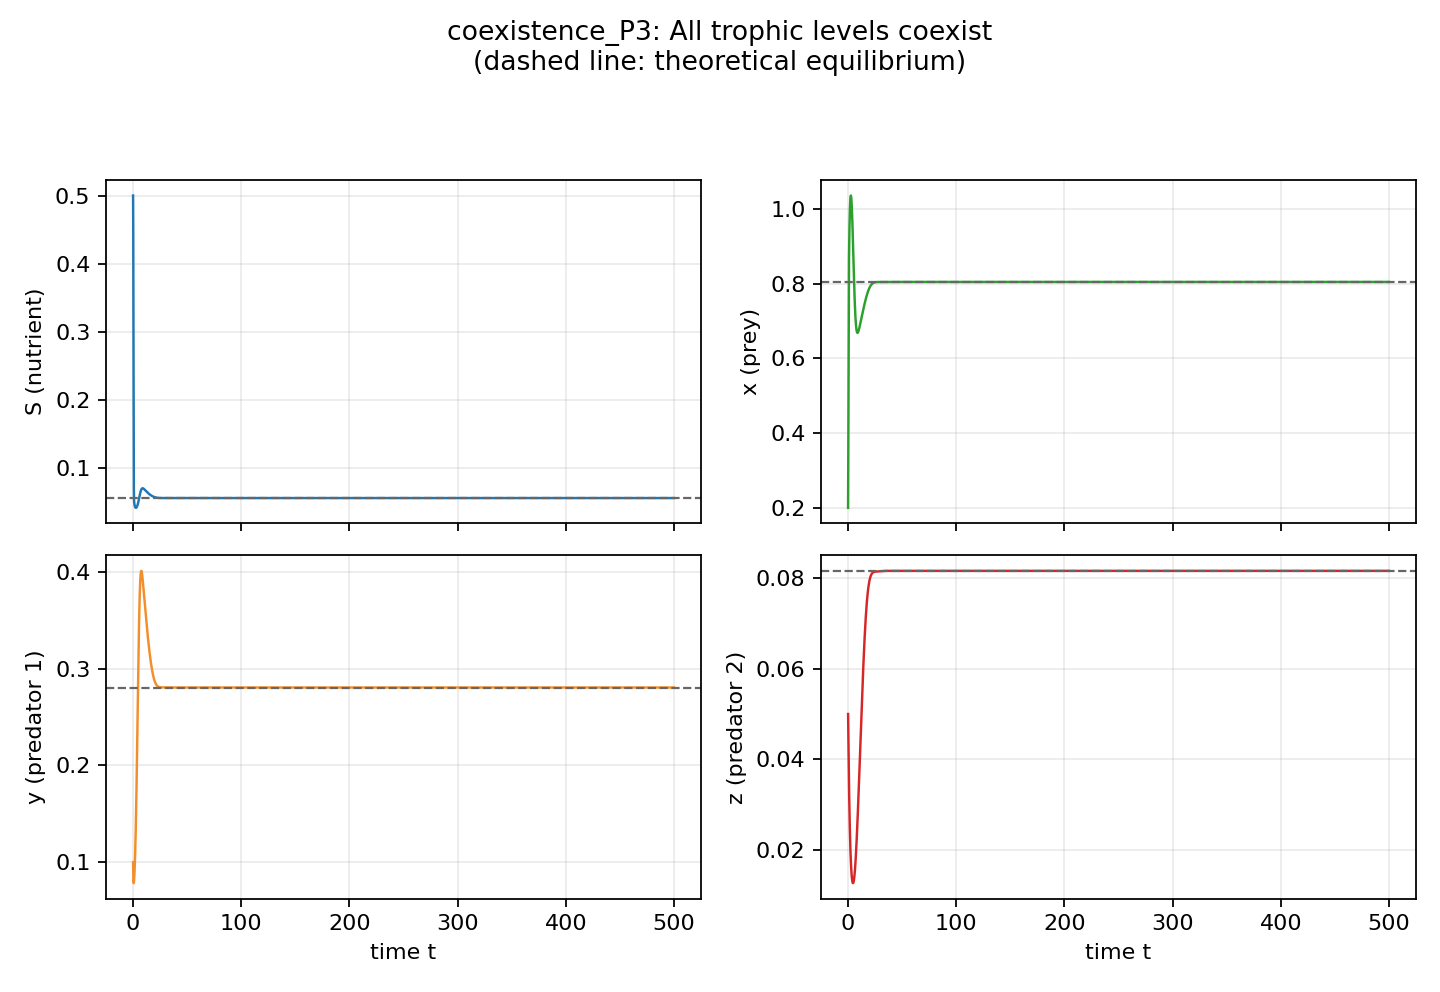
\includegraphics[width=0.88\textwidth]{results/main_scenarios/coexistence_P3_timeseries.png}
    \caption{Running simulation image for the coexistence scenario \(P_3\).}
    \label{fig:coexistence-p3-timeseries}
\end{figure}

\subsection{Oscillatory and Damped-Oscillatory Response}

The fifth scenario was included to demonstrate an interior response with
visible oscillations. Its analytical target equilibrium is
\[
P_3=(0.377311,0.540994,0.006908,0.001193).
\]
At \(t=2000\), the instantaneous numerical state was
\[
(S,x,y,z)\approx(0.377832,0.539609,0.008618,0.000146),
\]
with distance \(2.49\times 10^{-3}\) from \(P_3\). This final-state distance is
larger than in the previous cases because the endpoint depends on the phase of
the remaining oscillation.

To avoid misclassification, the oscillatory case was also evaluated using
window statistics. Over the late window \(1500\leq t\leq 2000\), the mean state
was only \(4.66\times 10^{-4}\) from \(P_3\). After \(t=500\), the trajectory
had 23 detected local maxima in \(y\) and 20 detected local maxima in \(z\).
The maximum ratio between the late-window amplitude and the middle-window
amplitude was 0.425, so the oscillations were decreasing. These measurements
identify the behavior as a slowly damped oscillatory approach to the interior
equilibrium. They are consistent with dynamics near a Hopf stability boundary,
but they do not by themselves prove a Hopf bifurcation.

\begin{figure}[htbp]
    \centering
    
\includegraphics[width=0.88\textwidth]{results/main_scenarios/oscillatory_interior_response_timeseries.png}
    \caption{Running simulation image for the slowly damped oscillatory scenario.}
    \label{fig:oscillatory-timeseries}
\end{figure}

\begin{figure}[htbp]
    \centering
    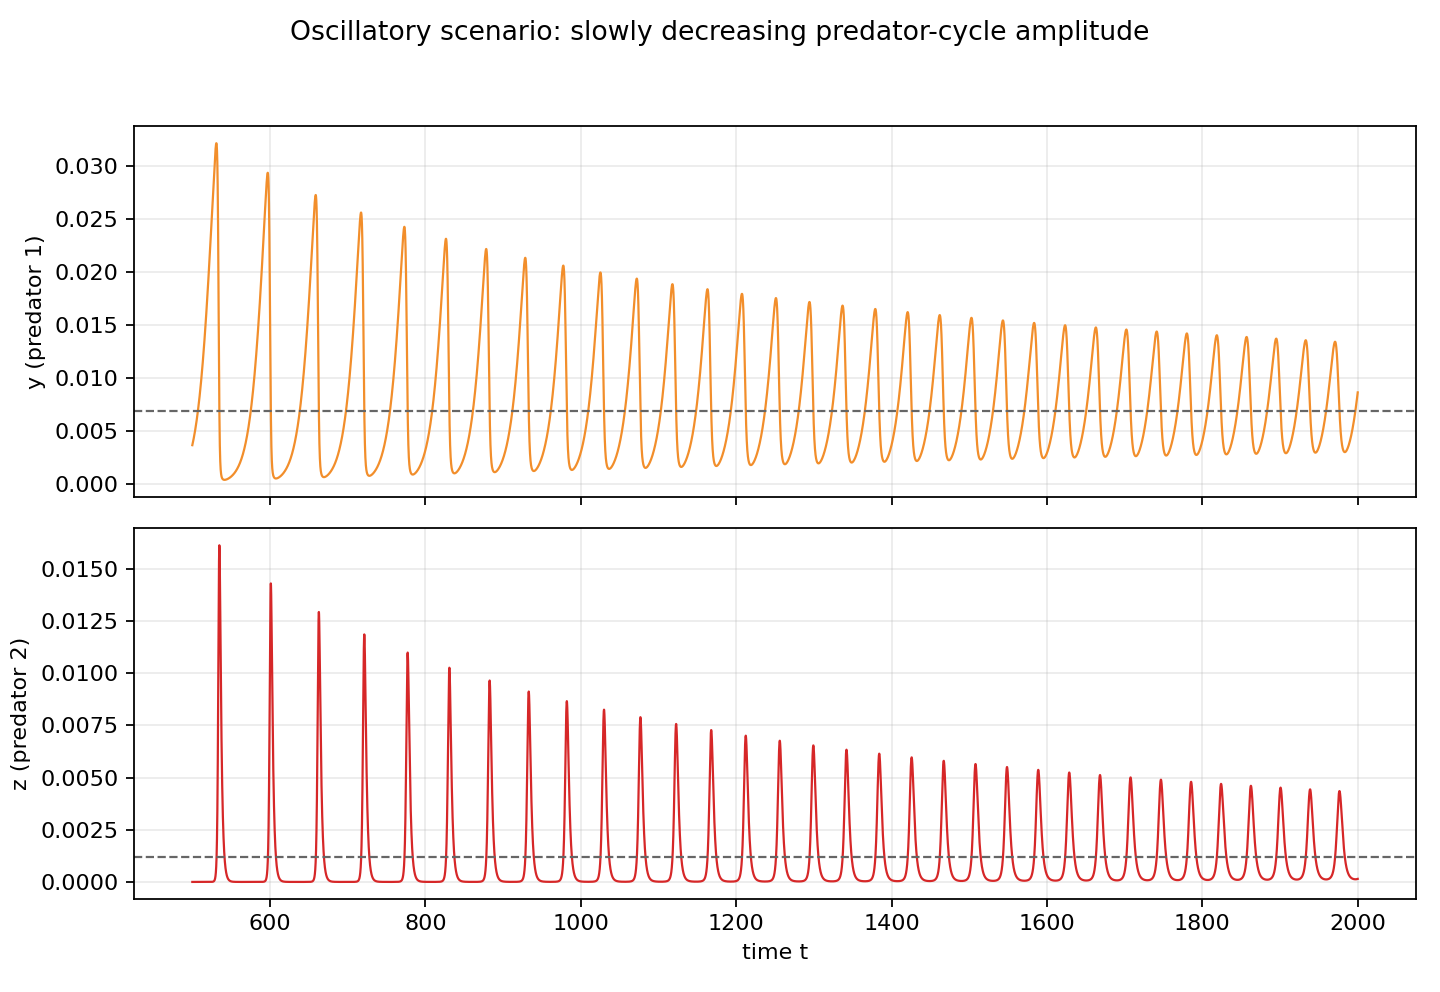
\includegraphics[width=0.88\textwidth]{results/main_scenarios/oscillatory_interior_response_zoom.png}
    \caption{Zoomed view of the predator oscillations after the initial transient.}
    \label{fig:oscillatory-zoom}
\end{figure}

\subsection{Comparison Between Numerical and Theoretical Equilibria}

Table~\ref{tab:numerical-theoretical-comparison} compares the numerical final
states with their theoretical targets. The first four experiments agree with
their expected equilibria to high accuracy. The oscillatory case is naturally
less well represented by a single final point, so its window average was used
as the main evidence for convergence toward \(P_3\).

\begin{table}[htbp]
\centering
\caption{Comparison between numerical final states and theoretical equilibria.}
\label{tab:numerical-theoretical-comparison}
\begin{tabular}{lllc}
\hline
Scenario & Target & Numerical final state \((S,x,y,z)\) & Distance\\
\hline
\(P_0\) washout & \(P_0\) & \((1.000000,0,0,0)\) & \(5.55\times 10^{-15}\)\\
\(P_1\) prey only & \(P_1\) & \((0.166667,1.666667,0,0)\) & \(2.57\times 10^{-14}\)\\
\(P_2\) two species & \(P_2\) & \((0.628666,0.333334,0.409333,0)\) & \(1.29\times 10^{-6}\)\\
\(P_3\) coexistence & \(P_3\) & \((0.055067,0.804597,0.280534,0.081550)\) & \(1.94\times 10^{-11}\)\\
Oscillatory response & \(P_3\) & \((0.377832,0.539609,0.008618,0.000146)\) & \(2.49\times 10^{-3}\)\\
\hline
\end{tabular}
\end{table}

\subsection{Biological Interpretation of the Results}

The simulations show a clear trophic survival hierarchy. In \(P_0\), the prey
cannot overcome removal, so the entire biological chain washes out. In \(P_1\),
the prey survives but does not create enough food supply for predators. In
\(P_2\), the first predator persists, but the top predator cannot invade. In
\(P_3\), all trophic levels have sufficient effective growth relative to their
removal rates, so the system settles at a positive coexistence equilibrium.

The main biological mechanism is therefore the balance between food-dependent
growth and species-specific removal. Each higher trophic level can persist
only if the lower level maintains a concentration high enough to make the
corresponding Monod response exceed the removal rate. The numerical results
also show why long simulations and analytical equilibria should be used
together. Graphs reveal transient oscillations, while equilibrium distances
give a quantitative test of the predicted long-term regime.

\subsection{Interactive Simulator Demonstration}

The project also includes an interactive browser simulator in the
\texttt{demo/} directory. It can be launched from the repository root by
running
\[
\texttt{python -m demo.app}
\]
and then opening \(\texttt{http://127.0.0.1:8000}\) in a browser. The
interface allows the user to choose scenario presets, change the removal
rates \(D_1,D_2,D_3\), adjust the Monod parameters, and observe the RK4
trajectory in real time. It also displays analytical equilibria, invasion
thresholds, local stability information, and the nearest equilibrium to the
current live state. This makes the simulation results easier to interpret
during the presentation because the audience can see how changing a removal
rate moves the system between washout, partial survival, and coexistence.

\begin{figure}[htbp]
    \centering
    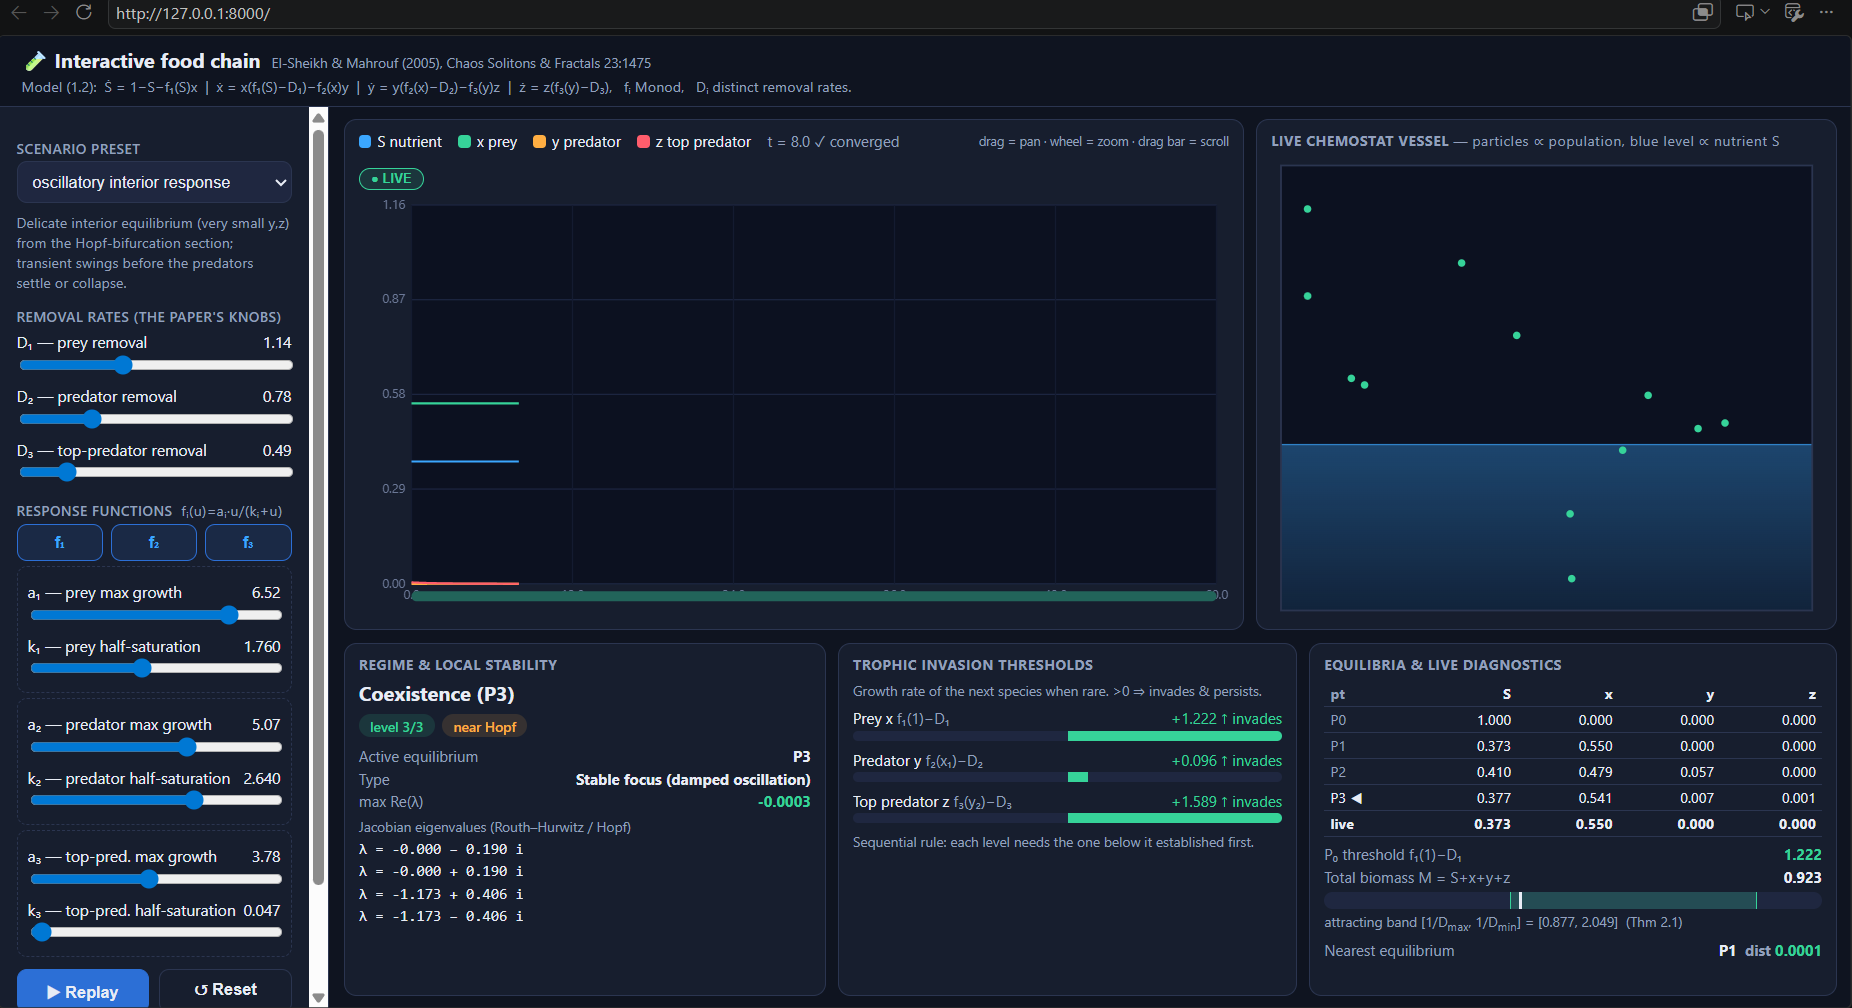
\includegraphics[width=1\textwidth]{images/UI.png}
    \caption{Screenshot of the interactive simulator showing live trajectories, parameter sliders, equilibrium table, and stability diagnostics.}
    \label{fig:interactive-simulator-demo}
\end{figure}

\tocsection{Sensitivity Analysis}
\tocsubsection{Sensitivity-Analysis Design}
\tocsubsection{Removal-Rate Sweep for D1}
\tocsubsection{Removal-Rate Sweep for D2}
\tocsubsection{Removal-Rate Sweep for D3}
\tocsubsection{Elasticity Coefficients}
\tocsubsection{Interpretation of Sensitive Parameters and Thresholds}

\tocsection{Robustness Analysis}
\tocsubsection{Time-Step and Solver Robustness}
\tocsubsection{Initial-Condition Robustness}
\tocsubsection{Agreement Between Theory and Simulation}
\tocsubsection{Numerical and Modeling Limitations}

\tocsection{Conclusions}
\tocsubsection{Main Conclusions from the Reference}
\tocsubsection{Conclusions from the Reimplemented Simulator}
\tocsubsection{Limitations and Possible Extensions}

\tocunnumberedsection{References}


\end{document}
